\documentclass{article}
\usepackage[utf8]{inputenc}
\usepackage[brazil]{babel}

\title{UTFPR - Engenharia de Computação\\
		IF61B - Algoritmos - C11-2016/1\\
		Atividade Prática Supervisionada - 00/00/2016}
\author{Monitor: Rafael Sian de Freitas }
\date{Maio 2016}

\usepackage{natbib}
\usepackage{graphicx}

\begin{document}

\maketitle

\section{Jogo do Bicho}
Visando aumentar os lucros do zoológico do Rio de Janeiro o Barão de Drummond criou o jogo do bicho, onde cada visitante que comprasse uma entrada poderia escolher um dos 25 bichos do zoológico para participar do jogo. Cada animal era associado a quatro números em sequência da seguinte forma: o primeiro animal (avestruz) é associado aos números 01, 02, 03 e 04; o segundo animal (águia) é associado aos números 05, 06, 07 e 08; e assim em diante até o último animal (vaca) que é associado com os números 97, 98, 99 e 00. Por mais que a legislação brasileira considere o jogo ilegal ele está presente no nosso cotidiano desde o século XIX. 

Existem vários modos de apostas no jogo do bicho, a mais popular é o Modo Simples de Aposta (conhecido também como "Na Cabeça"). Esse modo consiste em quatro sub-modos de apostas, que são as seguintes:

\begin{itemize}
	\item \textbf{Grupo} Você escolhe um animal e se um dos números que fazem parte do grupo desse animal sai na dezena do número sorteado você ganha 18 vezes o valor apostado.\\\\
	Ex.: Quem apostou 1,00 no cachorro e o número sorteado foi \textbf{56317} ganhou 18,00. 
	
	\item \textbf{Dezena} Você escolhe uma dezena qualquer, e se ela cair na dezena do número sorteado você ganha 60 vezes o valor apostado.\\\\
	Ex.: Quem apostou 3,00 no número 66 e o número sorteado foi \textbf{25166} ganhou 180,00. 
	
	\item \textbf{Centena} Você escolhe uma centena qualquer, e se ela cair na centena do número sorteado você ganha 600 vezes o valor apostado.\\\\
	Ex.: Quem apostou 2,00 no número 123 e o número sorteado foi \textbf{85123} ganhou 1200,00. 
	
	\item \textbf{Milhar} Funciona da mesma maneira da dezena e centena, você escolhe um milhar qualquer e se esse número cair no número sorteado você ganha 4000 vezes o valor apostado.\\\\
	Ex.: Quem apostou 5,00 no número 4567 e o número sorteado foi \textbf{194567} ganhou 20000,00. 
	
	\item Caso nenhum dos casos acima ocorrer, o apostador não recebe nada.
\end{itemize}

Para apostar no Jogo do Bicho é bem simples, basta você escolher o modo de aposta, um sub-modo \textbf{SM}, valor da aposta \textbf{V} e um número \textbf{N} (0 < N < 1000000). Após isso é sorteado um número \textbf{M} (0 < M < 1000000) e assim é verificado os resultados de cada apostador de acordo com o sub-modo escolhido. Caso o número apostado ou o sorteado tenha menos que quatro dígitos, são adicionados dígitos 0 na frente do número para que se torne de quatro dígitos; por exemplo, 66 corresponde a 0066;

\subsection{Entrada}
Dado o valor da aposta, o número escolhido pelo apostador e o sub-modo, seu programa deve calcular um número aleatório menor que 1000000 e exibir o prêmio do apostador. Além disso, o programa deve ficar calculando prêmios com as suas respectivas entradas até o usuário digitar -1 na entrada do valor da aposta.

\subsection{Saída}
Para cada prêmio calculado deve ser mostrado o valor da aposta e o valor do prêmio recebido, ambos com duas casas decimais, o sub-modo escolhido, o número escolhido pelo apostador, o número sorteado pelo programa e o bicho que deu com base na dezena do número sorteado (consultar tabela abaixo para verificar os grupos de animais).

\begin{figure}[!h]
	\centering
	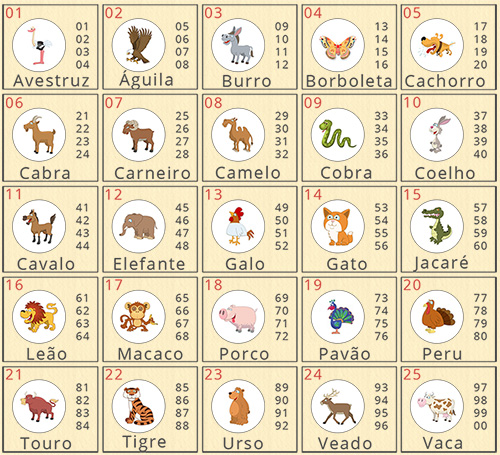
\includegraphics[scale=0.5]{tabela-de-resultados.jpg}
	\caption{Tabela com os números dos animais}
\end{figure}

\subsection{Regras}
\begin{itemize}
	\item Não pode usar vetor ou string para ler a entrada do número do apostador;
	\item Os intervalos do número do apostador deve estar dentro do limite definido (0 < N < 1000000)
\end{itemize}

\subsection{Dicas}
\begin{itemize}
	\item Colocar o \textit{seed} do random com o valor da hora do sistema: \textbf{srand(time(NULL))}
\end{itemize}

Abaixo estão \textbf{exemplos} de entradas e as suas respectivas saídas.\\

\noindent\fbox{%
	\parbox{\textwidth}{%
		\textbf{Entrada 1}\\
		Valor da aposta: 5.00\\
		Número escolhido: 18\\
		Sub-modo: grupo\\
		
		\textbf{Saída 1}\\
		Valor da aposta: 5.00\\
		Número escolhido: 18\\
		Sub-modo: grupo\\
		Número sorteado: 14020\\
		Prêmio: 90.00\\
		Bicho: Cachorro
	}%
}\\\\

\noindent\fbox{%
	\parbox{\textwidth}{%
		\textbf{Entrada 2}\\
		Valor da aposta: 20.00\\
		Número escolhido: 1256\\
		Sub-modo: dezena\\
		
		\textbf{Saída 2}\\
		Valor da aposta: 20.00\\
		Número escolhido: 1256\\
		Sub-modo: dezena\\
		Número sorteado: 0056\\
		Prêmio: 1200.00\\
		Bicho: Gato
	}%
}\\\\

\noindent\fbox{%
	\parbox{\textwidth}{%
		\textbf{Entrada 3}\\
		Valor da aposta: 521.00\\
		Número escolhido: 21355\\
		Sub-modo: centena\\
		
		\textbf{Saída 3}\\
		Valor da aposta: 521.00\\
		Número escolhido: 21355\\
		Sub-modo: centena\\
		Número sorteado: 13355\\
		Prêmio: 312600.00\\
		Bicho: Gato
	}%
}\\\\

\noindent\fbox{%
	\parbox{\textwidth}{%
		\textbf{Entrada 4}\\
		Valor da aposta: 38.30\\
		Número escolhido: 32\\
		Sub-modo: milhar\\
		
		\textbf{Saída 4}\\
		Valor da aposta: 38.30\\
		Número escolhido: 6332\\
		Sub-modo: milhar\\
		Número sorteado: 5596332\\
		Prêmio: 153200.00\\
		Bicho: Camelo
	}%
}\\\\

\newpage
\section{Correção de simulado}
Todo final de semestre em uma escola é aplicado um simulado sobre toda a matéria do semestre. O simulado contém N questões com 5 alternativas cada e somente uma das alternativas é a correta. O simulado é corrigido um por um pelos professores que além disso também fazem uma estatística do simulado que mostram:

\begin{itemize}
	\item \textbf{Maior nota entre os alunos}
	\item \textbf{Menor nota entre os alunos}
	\item \textbf{Percentual que cada questão teve}
\end{itemize}

A nota final do aluno é a quantidade de questões acertadas, sendo que todas tem o mesmo peso.\\

Pensando na otimização da correção desse simulado foi requisitado que você faça um programa em C para automatizar a correção. 

\subsection{Entrada}
O gabarito deve ser preenchido com respostas válidas (de 1 até 5) até o usuário digitar o número 0. A quantidade de questões será baseado no tamanho do gabarito, sendo que o programa vai aceitar as respostas válidas (de 1 até 5) para cada questão até completar o tamanho do gabarito. O número de alunos será informado no inicio do programa.

\subsection{Saída}
Para cada aluno será calculado a nota que ele obteve no simulado, mostrando a quantidade de questões acertadas e erradas. No final disso deve ser mostrado as estatísticas que os professores fazem: maior nota; menor nota; percentual que cada questão teve. 

\subsection{Regras}
\begin{itemize}
	\item Deve ser utilizado uma matriz para armazenar as respostas do alunos.
	\item Deve ser utilizado um vetor para armazenar o gabarito das respostas corretas.
	\item O calculo do percentual de que cada questão teve deve ser feito através de uma função que receberá a quantidade de alunos que acertaram uma determinada questão e o total de alunos que realizaram o simulado. Só deve ser mostrado duas casas decimais do percentual.
	\item Deve ser utilizados os comandos \textbf{continue} e \textbf{break}.
\end{itemize}

\subsection{Dicas}
\begin{itemize}
	\item Utilize a diretiva \textbf{\#define} para facilitar os testes no programa.
	\item Para efeitos de teste você pode gerar números randômicos (que sigam as regras) para preencher a matriz dos alunos. Fazendo isso você não vai precisar digitar os números no teclado. 
\end{itemize}

Abaixo estão \textbf{exemplos} de entradas e as suas respectivas saídas.\\

\noindent\fbox{%
	\parbox{\textwidth}{%
		
	\textbf{Entrada}\\\\
	Quantidade de alunos: 3\\
	Gabarito:

	\begin{tabular}{| l | l | l | l | l | l | l | l |}
		\hline
		1 & 1 & 3 & 5 & 4 & 3 & 2 & 0 \\
		\hline
	\end{tabular}\\
	
	Matriz de alunos com as questões:
	
	\begin{tabular}{| l | l | l | l | l | l | l |}
		\hline
		1 & 1 & 2 & 1 & 4 & 3 & 2 \\
		\hline
		2 & 1 & 4 & 1 & 4 & 3 & 2 \\
		\hline
		3 & 2 & 3 & 4 & 4 & 2 & 1 \\
		\hline
	\end{tabular}\\\\

		
	\textbf{Saída}\\
	Aluno 1: acertou 5 de 7\\ 
	Aluno 2: acertou 4 de 7\\
	Aluno 3: acertou 1 de 7\\

	A maior nota foi: do aluno 1 (5 de 7)\\
	A menor nota foi: do aluno 3 (1 de 7)\\
	
	Percentual de acertos:\\
	
	Questão 1: 33,34\% de acerto\\
	Questão 2: 66,67\% de acerto\\
	Questão 3: 33,34\% de acerto\\
	Questão 4: 0,00\% de acerto\\
	Questão 5: 100,00\% de acerto\\
	Questão 6: 66,67\% de acerto\\
	Questão 7: 66,67\% de acerto\\
	}%

}

\end{document}
